% -*- mode: latex -*-

\week[description={Last week we discussed information. This week we start to understand that combining information with decision making is the foundation on which we can build complex behaviors.}]{Making Decisions}

\resource[silent,files={motherduck.html},description={Play the DuckBot game online},text={DuckBot}]{demos/duckbot.html}
\resourcegen{name=data/duckbot.tar.gz, type={archive}, from={week3 game.py sample_brain.py assets/tileset.json assets/maps/level1.json assets/maps/level2.json assets/maps/level3.json assets/maps/level4.json assets/duck.png assets/terrain_atlas.png}}
\resourcegen{name=demos/duckbot.html, from=week3/site/duckbot.html, type={jinja}}

The ancient Greek polymath Eratosthenes regularly traveled between the Egyptian cities of Syene and
Alexandria (see \prettyref{fig:alexandria}). He was a very observant scientist, and -- like many
ancient polymaths -- was interested in astronomy. He noticed that, on the summer solstice, the
following things were true (see \prettyref{fig:eratosthenes}):
\begin{marginfigure}
  \centering
  \includegraphics[width=0.9\marginparwidth]{../week3/figures/syene-alexandria.jpg}

  \caption{The distance between the Egyptian cities of Alexandria and Syene is 5000 stadia or approximately 787.5 kilometers apart.}
  \label{fig:alexandria}
\end{marginfigure}

\begin{enumerate}
\item In Syene, which was south of Alexandria, on the summer solstice, the sun shone straight down. If he looked at the bottom of a deep well, there were no shadows at all. If you planted a stick in the ground, the stick would cast no shadow, because the sun was directly overhead.
\item In Alexandria, to the north, on the same day at the same time, if you planted a stick in the ground, there was a shadow.
\end{enumerate}

What can be deduced based off these two observations?

Here's some more details: the straight-line distance between the two cities is approximately 787.5
kilometers apart. Also, the angle of the shadow cast on the ground in Alexandria was $7.5^{\circ}$.

Eratosthenes did the following calculation:

\[
\underbrace{787.5\;\text{kilometers}}_{\text{distance between the two cities}} \times \frac{360^{\circ}}{7.5^{\circ}} \approx 40,000\;\text{kilometers}
\]

\begin{figure}
  \centering

  \begin{tikzpicture}[scale=0.5,font={\sffamily}]
    \node at (0, 10) {Sun};
    \draw (0, 10) circle (1);
    \draw (-2, 0) -- (10, 0) node[midway, anchor=north, yshift=-0.1em] {Ground};

    \draw (0,0) -- (0, 4);

    \coordinate (alexandria bottom) at (6, 0);
    \coordinate (alexandria stick) at (6, 4);

    \path[name path=ray] (alexandria stick) -- ++(-82.5:100);
    \path[name path=x axis] (-10, 0) -- (10, 0);
    \fill[name intersections={of=ray and x axis, by=B}, dashed, fill=lightgray]
      (alexandria bottom) -- (alexandria stick) -- (B);
    \draw (alexandria bottom) -- (alexandria stick);
    \draw[dashed] (alexandria stick) -- (B);
    \draw[ultra thick] (B) -- (alexandria bottom);

  \end{tikzpicture}

  \caption{Eratosthenes noticed that on the summer solstice the shadows cast by the Sun at noon appeared different in two cities. In Syene, there was no shadow, which meant the Sun was directly overhead. In Alexandria, there was a shadow.}
  \label{fig:eratosthenes}
\end{figure}

\didyouknow{
Albert Einstein famously came up with his theory of special relativity by simply thinking about it!
If you ever study physics in depth, you'll discover that the entirety of special relativity falls
out of two simple facts:
\begin{enumerate}
\item The speed of light is the same for everyone.
\item The relationship between the sides of the triangle: $c^2 = a^2 + b^2$.
\end{enumerate}
Einstein used these simple facts to show that light actually travels less distance in moving
reference frames, leading to one of the most surprising facts about our universe: fast things become
shorter.  }
\begin{BigIdeaBox}
As humans, we only see our part of the world and our part of the universe. The consistent
application of precise rules lets us reason about things larger than what we can directly perceive.

Despite having no possible way to observe the entirety of the planet. Eratosthenes used simple rules
of logic and simple observations to deduce a global truth.
\end{BigIdeaBox}

\section{Week 2 Review}

Last week, we discussed breaking down large drawings and objects into smaller elements. Doing so let
us build large drawings from simple drawings we could combine together. Even though the set of
simple or \term{primitive} drawings were small, we could draw quite a bit with them.

\section{Understanding Big Things}

The Turtle cursor we saw last week simply knew what was around it. We gave it commands based on its
\emph{immediate} environment and based on those, it simply followed what we told it. It was up to us
to give it the set of rules necessary to make the drawings we wanted. On its own, it was unable to
decide what to do.

When we programmed Turtle, we would run a function, draw it, and see what it looked like and where
the cursor ended up. Based on that, we would add another line or circle to our drawing. This process
involves a human (you) deciding what to do after each step.

Of course, in real life, computers do not wait for human input for every decision. Rather, they make
them on their own using long sets of rules that computer programmers assemble for the
computer. These rules have to be very detailed so that the computer knows what to do in every
possible situation it may encounter. Unlike with Turtle, there's no one around to change course if
the cursor ends up in the wrong spot or in the wrong orientation. Lists of rules that computers
follow on their own without human input is called an \term{algorithm}.  \didyouknow{The word
  \emph{algorithm} comes from the name of the Persian polymath and mathematician
  al-Khw\={a}rizm\={i} who introduced the idea of algorithms to the West via his book
  \emph{kit\={a}b al-\d{h}is\={a}b al-hind\={i}} (``Book of Indian Computation''). This book was
  translated into Latin by Robert Chester in 1145, and was the principal mathematics textbook used
  in many universities for almost four centuries. Many of our modern methods of addition,
  subtraction, division, and multiplication come from his translations!
\vspace{1em}
\begin{center}
  \includegraphics[width=0.6\marginparwidth]{../week3/figures/al-kwharizmi.jpg}
\end{center}}


\section{Algorithms}

You're probably familiar with several types of algorithms already. For example, there's an algorithm
for adding and subtracting numbers. Similarly, there are strict sets of rules to follow for
multiplying numbers. Beyond mathematics, even everyday situations involve algorithms. Consider a
complicated intersection. Cars go based off of whether the lights are red or green. The lights
operate on their own according to pre-set instructions; there's no human involvement. The system
requires every car to follow the rules. Otherwise, the cars literally crash.

Thermostats are another example of an algorithm you use and interact with. Thermostats operate on
conceptually simple rules:

\begin{enumerate}
\item If the temperature is above the set maximum temperature, then start the AC unit.
\item If the temperature is between the set minimum and maximum temperature, turn everything off.
\item If the temperature is below the set minimum, then start the heater.
\end{enumerate}

These three simple rules result in a comfortable environment for everyone.

Our Turtle drawings from last weeks are also examples of simple algorithms. These algorithms
followed a sequence of rules in order to do something -- in our case, to draw a duck. But
oftentimes, algorithms have to decide to do something based off data. These are the kinds of
algorithms we will explore this week.

In order to learn and understand algorithms, we are going to play a simple game. But be
warned... this is not like any game you've played before!

\section{Introducing DuckBot!}

Meet DuckBot! DuckBot has been put in change of a group of three very silly little ducklings while
Mother Duck has gone away. But those naughty little ducklings have fried DuckBot's brain and have run
off. They are now hiding in some corner of the pond. DuckBot needs to find the ducklings before
Mother Duck gets back.

Your job is to give DuckBot a new brain so that it can find the ducklings!

Oh and one more thing: if DuckBot runs into any obstacle, like a rock, a plant, or the ground,
DuckBot dies and will never be able to make it to the ducklings. Your brain has to make sure he only
ever swims in water.

The DuckBot game window (see \prettyref{fig:duckbot}) has four parts:
\begin{enumerate}
\item This shows you where DuckBot is in the pond. You can change your view of the pond by using the
  arrow keys or dragging around with your mouse. You can zoom in or out using the mouse wheel or the
  \litkey{+} and \litkey{-} keys. But remember, whatever you can see doesn't matter, because DuckBot
  can only see what's immediately around it.

\item The brain pane shows you the current Python code in DuckBot's brain. DuckBot runs this code
  each time it moves a square in the pond, in order to decide what to do next. You can edit the code
  here to make DuckBot do what you want.

\item This status panel tells you the current status of DuckBot. Any
  error messages caused by your Python code will appear here.

\item The controls pane lets you control DuckBot. You can make DuckBot go or stop by clicking the ``Start Duck'' and ``Stop Duck'' buttons. You can reset the game by clicking the ``Reset Game'' button.\hint{You'll need to stop the duck before resetting the game or reloading DuckBot's brain} When you've made changes to your brain, you have to tell DuckBot to switch to the new brain by clicking the ``Reload Brain'' button.

\item The bottom pane shows you what DuckBot sees. DuckBot can see obstacles in all four cardinal
  directions. You can also change DuckBot's speed here or choose to have DuckBot make just one step.

\end{enumerate}

\begin{figure}
  \centering
  \includegraphics[width=0.9\linewidth]{../week3/figures/duckbot.jpg}
  \caption{The DuckBot interface has five main components: (1) the pond, (2) the brain source code, (3) the error window, (4) the controls, and (5) the state window}
  \label{fig:duckbot}
\end{figure}

\subsection{The Pond}

The pond is where DuckBot and the ducklings live. It is divided into squares. Some squares are
passable, and others have obstacles (\prettyref{fig:obstacles}). DuckBot cannot swim over the
obstacles, and if your brain program tells it to swim into an obstacle DuckBot will die. You must
avoid all obstacles.

\begin{marginfigure}
  \centering
  \includegraphics[width=0.9\marginparwidth]{../week3/figures/obstacles.jpg}
  \caption{Examples of obstacles are rocks, weeds, and piers. You can always know if a square is an
    obstacle based on DuckBot's senses. Remember, the goal is for you to tell DuckBot what to do by
    writing a program, not for you to navigate around the pond yourself.}
  \label{fig:obstacles}
\end{marginfigure}

When you swim over a pond square that is filled with water, the square will become darker,
indicating that DuckBot has already been there. These dark squares are only visible to you, the
programmer. DuckBot cannot change its behavior based on whether it's visited a square or
not. DuckBot can only sense whether the squares around it have any obstacles in the way.

\subsection{Programming DuckBot}

DuckBot is programmed in Python. The goal of the game is to write a program so that DuckBot swims
over \emph{every} portion of the pond it can reach. The ducklings are \emph{very} sneaky and always
stay in the spot in which DuckBot is least likely to find them. Thus, DuckBot really must visit
every single portion of the pond.

The pond is arranged in a grid. DuckBot moves one square at a time. Once a square on the grid has
been swam over it turns darker, but DuckBot cannot see if it's already swam over a particular
square. It only sees what's around it and responds.

Every time DuckBot moves to a new square, the brain code is run again. The brain decides two things:

\begin{enumerate}

\item The \textbf{direction} that DuckBot ought to go in next.

\item The \textbf{thought} that DuckBot ought to think.

\end{enumerate}

DuckBot's brain is written as a function.

% TODO figure showing the function declaration
\begin{minipage}{\textwidth}
  \tikzforeground{
    \CheckTikzPictureSide
    \node[anchor=east] (brain function note) at ([yshift=5em, xshift={\tikztuftetowardsmargin * 1em}]current page text area.\tikztuftemain|-brain function name.north) {
      \begin{tcolorbox}[code note, width=4cm]
        Your function should be named \code{brain}.
      \end{tcolorbox}
    };
    \draw[->] (brain function note.south) to[out=-90,in=90,looseness=0.8] ([yshift=1em]brain function name.north);
  }
  \Large \ttfamily
  \vspace{0.5cm}
  \begin{tcolorbox}[sharp corners]
    \kw{def} \tikzmarknode{brain function name}{brain}(\tikzmarknode{north arg}{north}, \tikzmarknode{south arg}{south}, \tikzmarknode{east arg}{east}, \tikzmarknode{west arg}{west},\\
    \hspace{5em}\tikzmarknode{thought arg}{thought}):
  \end{tcolorbox}
\end{minipage}

\subsection{How DuckBot Perceives the World}

DuckBot can sense the four squares immediately to the north, south, east, and west of its current
location.\hint{Remember that Python requires us to surround letters and words in quotation marks.} A
blocked square is signified by the letter \code{'x'}. A free square is signified by the
letter \code{'*'}. This is illustrated in \prettyref{fig:duckbot-directions}.

DuckBot's brain is totally fried and so is its memory. DuckBot can only remember the last thing you
told it. This is called its \emph{thought}.\curious{DuckBot's thought is an example of
  \term{state}.} DuckBot can see what's around it in the current square. Based off of this knowledge
\emph{and} its previous thought, DuckBot has to decide the next direction and its next thought.

\begin{marginfigure}
  \centering
  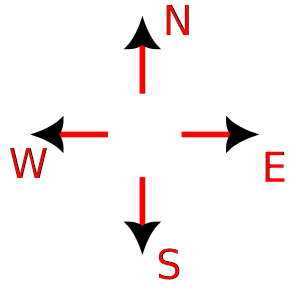
\includegraphics[width=0.8\marginparwidth]{../week3/figures/duckbot-directions.pdf}
  \caption{In this situation, DuckBot senses two free squares to the north (N) and west (W), and two blocked cells to the south (S) and east (E).}
  \label{fig:duckbot-directions}
\end{marginfigure}
You can see DuckBot's current thought in the information pane beneath the pond. When you first start
DuckBot, its thought is the number $0$.

In order to make DuckBot \emph{do} something, you have to give it instructions. Just like we saw
last week, to send data out of a function we use \kw{return}.

\begin{minipage}{\textwidth}
  \Large \ttfamily
  \tikzforeground{
    \node[anchor=\tikztuftemarg](return comma note) at ([xshift={\tikztuftetowardsmargin * 0.5cm},yshift=2cm]current page text area.\tikztuftemain|-return comma.north) {
      \begin{tcolorbox}[code note, width=4cm]
        The \code{,} (comma) tells \kw{return} that we are going to send back more than one piece of data.
      \end{tcolorbox}
    };

    \draw[->] (return comma note.\tikztuftemarg) to[out={acos(\tikztuftetowardsmargin)}, in=90] ([yshift=0.5em,xshift=0.5em]return comma.north);
  }
  \vspace{0.5cm}
  \begin{tcolorbox}[sharp corners]
    \tikzmarknode{return dir}{\kw{return}} \tikzmarknode{return direction}{'N'}\tikzmarknode{return comma}{,} \tikzmarknode{return next thought}{'next\_thought'}
  \end{tcolorbox}
\end{minipage}

This time, instead of just returning one thing, we're returning two
things. The first thing we return is which direction we want DuckBot
to go in. This can be:

\begin{itemize}
\item \code{'N'} to go north
\item \code{'E'} to go east
\item \code{'S'} to go south
\item \code{'W'} to go west
\item \code{\kw{None}} to stay in the same place\hint{\kw{None} is a
  special Python value indicating the absence of any data. You don't
  need to put it in quotes. If you did, then you would get the string
  \code{'None'} instead of the special \code{None} value}
\end{itemize}

The second thing we return is DuckBot's next thought. The thought can be anything: a number or a
string or even the \code{None} value.\hint{You'll probably want your thoughts to mostly be
  strings. This will make your code easier to understand.} You get to decide!

\subsection{Playing the Game}

When you open DuckBot, load a new level or press the ``Reset Game'' button, the pond is cleared and
DuckBot and the ducklings end up in random parts of the pond.\curious{Actually, the ducklings end up
  in the pond you're least likely to end up in. That's why it's so important DuckBot hits the whole
  pond!}

\section{An Example DuckBot Level}

To make things clearer, let's try working through a single DuckBot level. The first level looks like
this:

% TODO duckbot level 1

DuckBot is placed at a random location. DuckBot's brain is the simple function:

\begin{lstlisting}
def brain(north, south, east, west, thought):
  return None, thought
\end{lstlisting}

What will happen if we start DuckBot with this brain? Let's try it. Click the ``Start Duck'' button
in the control pane (see \prettyref{fig:duckbot}). \hint{Remember, always try to \emph{predict} what
  is going to happen before we do anything on the computer.}

Hmm... that's no good. We want DuckBot to do something. Let's make DuckBot go east.

\hint{Remember to click the ``Reload Brain'' button to make DuckBot use the new brain.}
\begin{TryThisBox}
  Change DuckBot's brain to this:
  \begin{lstlisting}
def brain(north, south, east, west, thought):
  @@return 'E', thought@@
  \end{lstlisting}
\end{TryThisBox}

If you go ahead and run this, DuckBot will head all the way east until it hits the shore. Remember,
DuckBot is very fragile and does exactly what you tell it. If it hits land, it dies, which is what
happens here. We need to detect when there is an obstacle to the east and send DuckBot in a
different direction.

But, in order to do that, we need to figure out how to make our function \kw{return} one thing if
there is something to the east and \kw{return} another thing if not.

\subsection{Using \kw{if}}

\begin{marginfigure}
  \centering
  \includegraphics[width=0.9\marginparwidth]{../week3/figures/grace-hopper.jpg}
  \caption{Rear Admiral Grace Hopper was a famous computer scientist who invented a programming
    language called \term{COBOL} (\textbf{CO}mmon \textbf{B}usiness-\textbf{O}riented
    \textbf{L}anguage) which was one of the first to usewords like \kw{if} to define how programs
    ran. Before her innovation, computer programs were written using difficult machine code and
    obtuse mathematics. For her fundamental contributions to computer science, she was awarded the
    Presidential Medal of Freedom in 2016.}
  \label{fig:grace-hopper}
\end{marginfigure}

Python comes with a special word that does exactly what we want. This is called \kw{if}, and it works like this:

We write \kw{if} followed by a condition, and then a colon. If the condition is true, then the code
beneath the \kw{if} runs. If the condition is false, then all that code is skipped. This is
illustrated in \prettyref{fig:if-statement}.

\begin{figure}[b]
  \begin{minipage}{\linewidth}
    \Large \ttfamily

    \vspace{3em}
    \tikzforeground{
      \coordinate (condition brace start) at ([yshift=5.2em, xshift=0.4em]condition start);
      \coordinate (condition brace end) at ([yshift=5.2em]condition end);
      \draw[thick, decoration={brace, raise=0.2em}, decorate] (condition brace start) -- (condition brace end);
        \begin{tcolorbox}[code note]
          If this expression is \kw{True}, the part below the \kw{if} will run.
        \end{tcolorbox}
      };

      \coordinate (keyword if east) at ([xshift=15em]if keyword);
      \draw[thick, decoration={brace}, decorate] ([yshift=0.2em]keyword if east|-if keyword) -- ([yshift=0.2em]keyword if east|-else action) node[midway,anchor=west,xshift=0.5em,yshift=1em] {
        \begin{tcolorbox}[code note,width=4.5cm]
          These portions of \kw{if} are optional. Python applies conditions in the order they appear. If no portion of the \kw{if} applies because all the conditions are \kw{False}, then nothing happens.
        \end{tcolorbox}
      };
    }
    \begin{tcolorbox}[sharp corners]
      \tikzmarknode{if keyword}{\kw{if}} \tikzmarknode{condition start}{}north == '*'\tikzmarknode{condition end}{}:\\
      \tikzmarknode{if spaces}{\hspace{2em}}\tikzmarknode{action}{...}\\
      \tikzmarknode{elif keyword}{\kw{elif}} \tikzmarknode{elif condition start}{}south == '*'\tikzmarknode{elif condition end}{}:\\
      \hspace{2em}\tikzmarknode{elif action}{...}\\
      \tikzmarknode{else keyword}{\kw{else}} \tikzmarknode{no else condition}{:}\\
      \hspace{2em} \tikzmarknode{else action}{...}
    \end{tcolorbox}
  \end{minipage}
  \caption{The Python \kw{if} statement consists of several parts.}
  \label{fig:if-statement}
\end{figure}

To understand what it means to be ``beneath'' the \kw{if}, we have to understand how Python treats
the \code{:}. As we learned last week, Python is sensitive to how things are spaced out. When we
write \kw{def}, we have to put spaces to signify which code is part of our function. The same is
true of \kw{if}. \curious{The error thrown is called \code{IndentationError}.}If we want some code
to run when the condition is true, then all this code must be indented \emph{more} than the \kw{if}
statement. Moreover, all the code has to line up. If you indent one line with six spaces, and the
next line with ten, then Python will return an error.

Let's try using \kw{if} to make DuckBot do something if we have an obstacle to the east.

\hint{Note that it has \emph{two} equal signs. The double equal
  signs compares values. A single equal sign has a different meaning, which we'll explore later.}
\begin{TryThisBox}
  Change DuckBot's brain to this:
  \begin{lstlisting}
def brain(north, south, east, west, thought):
  @@if east == 'x':
    return 'N', thought@@
  return 'E', thought
  \end{lstlisting}
\end{TryThisBox}

Think about what's going to happen now. When you've decided what you think is going to happen to
DuckBot, hit ``Reload Brain'' and start DuckBot.

Uh-oh! DuckBot once again hit an obstacle, but this time it at least turned towards the north, once
it hit an obstacle to the east.

At this point, maybe it's a good idea to check if there's an obstacle to the north. But which
direction to turn then? North was left of east. We could go west, which is left of north.

Of course, if we did that, DuckBot would just go all the way to the west side of the pond, and hit
the wall there. We'll have to handle the west case as well. And then, if we turn south, DuckBot will
hit the bottom of the pond, so we have to turn back east.

\hint{This is one of those changes where it's really important that you try to \emph{predict} what
  is going to happen.}
\begin{TryThisBox}
  Change DuckBot's brain to this:
  \begin{lstlisting}[numbers=left,caption={A brain that checks for all obstacles},label={listing:duckbot-circle}]
def brain(north, south, east, west, thought):
  if east == 'x':
    return 'N', thought
  @@if north == 'x':
    return 'W', thought
  if west == 'x':
    return 'S', thought
  if south == 'x':
    return 'E', thought@@
  return 'E', thought
  \end{lstlisting}
\end{TryThisBox}

If you go ahead and try that, you'll find that poor DuckBot *still* hits the north shore. Clearly
we've not quite figured out how to make this work.

\begin{marginfigure}
  \centering
  \includegraphics[width=0.9\marginparwidth]{../week3/figures/duckbot-ne.jpg}
  \caption{The code in \prettyref{listing:duckbot-circle} may seem to work, but it is not careful
    enough to check for obstacles in every direction. DuckBot dies when it hits the north-east
    corner of the pond. You can see which obstacle DuckBot hit by looking at the darkened cattail
    weed to the north of DuckBot. Our code needs to be more careful.}
  \label{fig:duckbot-ne}
\end{marginfigure}

To understand what's going on, let's consider DuckBot at the northeast corner of the pond (see
\prettyref{fig:duckbot-ne}). At this point, \code{north} and \code{east} are \code{'x'} and
\code{south} and \code{west} are \code{'*'}. You can see this at the bottom left of the DuckBot
interface, which displays the current state of what DuckBot sees.

In the brain view, you'll also notice that some lines are highlighted. The lines highlighted in
light gray represent the code that was used by DuckBot to make its decision. The lines highlighted
in green represent points where decisions were made (i.e., places that used \kw{if}). Finally, the
line highlighted blue indicate where DuckBot made its decision.

If we look at the interface, we'll see that lines 2 and 3 (see \prettyref{listing:duckbot-circle})
are highlighted, indicating that these are what led to the decision DuckBot made. But that's not
what we wanted. We wanted DuckBot to make the decision to turn west, which is on line 5. The \kw{if}
of line 4 was supposed to check the condition that there was an obstacle to the north. But this line
is not highlighted, indicating it was not used. Why?

\curious{When Python encounters a \kw{return}, it ends the current function immediately. Thus it's
  important to properly consider the order of rules within a function.}  If you notice, the \kw{if}
that checked the obstacle to the east was used, and then, Python saw that there was an obstacle to
the east when DuckBot was in the northeast square. But, this \kw{if} has a \kw{return} under
it. Because the condition in the \kw{if} was true, Python used the code underneath it, which told
the function to immediately send back its decision to go north. This is not what we wanted. We have
to make sure that there's also no obstacle to the north.

\section{Booleans}

In the above code examples, we skipped over how we wrote the \kw{if} conditions, but it's worth
considering them in more detail right now. How does Python know whether a condition is true or not?
This is important to understand when Python is going to run code.

\begin{marginfigure}
  \centering
  \includegraphics[width=0.9\marginparwidth]{../week3/figures/george-boole.jpg}
  \caption{Booleans are named afetr \textbf{George Boole}, an English mathematician and
    philosopher. In 1854, Boole published a book \emph{The Laws of Thought} which formally
    introduced the Boolean values and made explicit the \kw{and} and \kw{or} operations.}
\end{marginfigure}

Try this in your Python prompt:

\begin{replbox}
>>> True
True
>>> False
False
\end{replbox}

These values are two special values used by Python to indicate -- as you'd expect -- whether
something is true or false. The collective term for these kinds of values is \term{booleans}.

Booleans can be combined using symbols, similar to addition and multiplication of numbers. For
example, the symbol \kw{and} checks if both sides are \kw{True}, and returns \kw{True} if they
are.

\begin{replbox}
>>> True and False
False
>>> True and True
True
>>> False and False
False
>>> False and True
False
\end{replbox}

The symbol \kw{or} checks if only one side is \kw{True}.

\begin{replbox}
>>> True or False
True
>>> True or True
True
>>> False or False
False
>>> False or True
True
\end{replbox}

There are only two possibilities for the values on each side of a \kw{and} or \kw{or}. Thus, there
are four possible combinations of values that can go into these symbols. We can write out the entire
set of inputs and outputs as a four-row table. These are called \term{truth tables}. The tables for
\kw{and} and \kw{or} are given in \prettyref{fig:and-or-truth-tables}.

\begin{figure}
  \begin{minipage}{0.45\textwidth}
    \begin{center}
      \begin{tabular}{cc|c}
        \multicolumn{3}{c}{\texttt{x}\;\kw{and}\;\texttt{y}} \\\hline
        \texttt{x} & \texttt{y} & \\\hline
        \kw{True} & \kw{True} & \kw{True} \\
        \kw{True} & \kw{False} & \kw{False} \\
        \kw{False} & \kw{True} & \kw{False} \\
        \kw{False} & \kw{False} & \kw{False} \\\hline
      \end{tabular}
    \end{center}
  \end{minipage}
  \begin{minipage}{0.45\textwidth}
    \begin{center}
      \begin{tabular}{cc|c}
        \multicolumn{3}{c}{\texttt{x}\;\kw{or}\;\texttt{y}} \\\hline
        \texttt{x} & \texttt{y} & \\\hline
        \kw{True} & \kw{True} & \kw{True} \\
        \kw{True} & \kw{False} & \kw{True} \\
        \kw{False} & \kw{True} & \kw{True} \\
        \kw{False} & \kw{False} & \kw{False} \\\hline
      \end{tabular}
    \end{center}
  \end{minipage}

  \caption{These are the truth tables for the \kw{and} and \kw{or} rules. The inputs are in the left two columns and the output is in the right. Try all of these in the Python prompt to verify that they work.}
  \label{fig:and-or-truth-tables}
\end{figure}

\subsection{Inspecting data}

The conditions that we've been using in our \code{brain} functions are an example of comparing
values. Python has several rules and symbols to compare values. We've been using \code{==} which
checks that two things are equal. There are other \term{operators} that check for other
conditions. For a full summary see \prettyref{tab:comparisons}.

\begin{table}[b]
  \centering
  \begin{tabular}{lp{0.8\linewidth}}
    \hline
    \headercol{Operator} & \headercol{Explanation} \\\hline
    \code{x == y} & Checks if \code{x} and \code{y} are equal. \\
    \code{x != y} & Checks if \code{x} and \code{y} are not equal. \\
    \code{x < y} & Checks if \code{x} is less than \code{y}. \\
    \code{x > y} & Checks if \code{x} is greater than \code{y}. \\
    \code{x <= y} & Checks if \code{x} is less than or equal to \code{y}. \\
    \code{x >= y} & Checks if \code{x} is greater than or equal to \code{y}. \\
    \code{x is None} & Checks if \code{x} is \kw{None} or empty. \\
    \code{x is not None} & Checks if \code{x} is not \kw{None}. \\\hline
  \end{tabular}
  \caption{Some Python operators that can be used to inspect data that return booleans. Note that
    for strings, \code{x < y} means that \code{x} comes before \code{y} in standard alphabetical
    order.}
  \label{tab:comparisons}
\end{table}

These rules result in booleans. Let's try it.

\begin{replbox}
>>> 'x' == 'x'
True
>>> 'x' == 'y'
False
>>> 4 < 5
True
>>> 4 >= 5
False
\end{replbox}

We can combine these using \kw{and} and \kw{or}

\begin{replbox}
>>> 4 < 5 and 5 <= 10
True
>>> 5 < 4 or 5 > 10
False
\end{replbox}

Going back to our brain above, we can now use \kw{and} to ensure that we do not continue north
simply because we are blocked to our east. Instead, we also check that north is free.

\begin{TryThisBox}
  Change DuckBot's brain to this:
  \begin{lstlisting}
def brain(north, south, east, west, thought):
  if east == 'x' @@and north == '*':@@
    return 'N', thought
  if north == 'x' @@and west == '*':@@
    return 'W', thought
  if west == 'x' @@and south == '*':@@
    return 'S', thought
  if south == 'x' @@and east == '*':@@
    return 'E', thought
  return 'E', thought
  \end{lstlisting}
\end{TryThisBox}

Let's try running this. That's much better -- DuckBot doesn't die. But it also looks like DuckBot is
stuck going in circles. Those ducklings won't be found unless DuckBot searches every square of the
pond. Can we figure out what's going on?

\subsection{Infinite Loops}

Consider what's happening here: although DuckBot no longer breaks, it also is not fully
working. \curious{DuckBot not breaking but also not being able to tell you that anything is wrong is
  an example of a kind of behavior that's broken but that Python cannot report as an error: there is
  no Python rule you are breaking. Python faithfully carries out exactly the rules you gave to it.}

Can we understand why? Let's once again, consider the case when DuckBot hits the north-east
corner. What do we want to happen? We currently turn left, towards the west, to prevent DuckBot from
dying by continuing to go north. Then, when DuckBot is going west, the only thing we ensure is that
DuckBot continues west until it can't go any further, at which point we turn left again. At some
point, this leads DuckBot right back to the north-east square, and the cycle repeats.\hint{The cycle
  repeats because there's no way for DuckBot to know if it's already visited that square
  before. Therefore, DuckBot \emph{has} to continue doing the same thing over and over and over
  again.}

If we want to fix this, we need to consider what \emph{ought} to happen when DuckBot hits this
corner. Obviously, we can't keep going west -- we tried that and it didn't work. What we really want
is DuckBot to go west one square, and then turn back south (see
\prettyref{fig:duckbot-desired-outcome}). That way it'll hit squares that are in the middle of thei
pond, not just on the perimeter.

If you step through the game, you'll notice that, after DuckBot turns at the north-east corner and
is going west, it no longer has any way to know it was at the north east corner. In order to know
that it needs to turn immediately after going west one square after it hits the corner, we need to
make DuckBot remember that it's planning on turning after it moves one block west. This is where
DuckBot's \code{thought} comes in.

\begin{marginfigure}
  \centering
  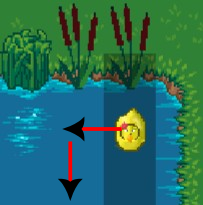
\includegraphics[width=0.9\marginparwidth]{../week3/figures/duckbot-ne-desired.jpg}
  \caption{When DuckBot reaches the northeast corner, we want it to turn west for only \emph{one}
    square, and then turn back south, but the environment one square to the west of the north east
    corner looks the same as all other squares at the northern border. Therefore, DuckBot needs to
    modify its \emph{thought} at the north east square so that it can distinguish the square
    immediately to the west of it from all the other squares.}
  \label{fig:duckbot-desired-outcome}
\end{marginfigure}

Recall that each time the \code{brain} function is used, it gets what DuckBot sees and also the last
thing DuckBot thought. In our previous brains, we just \kw{return}ed whatever it was that DuckBot
was already thinking. Now, we need to use that \code{thought} in order to remember what
happened. Let's try it.

\begin{TryThisBox}
  \label{trythisbox:sample-brain}
  Change DuckBot's brain to this:
  \begin{lstlisting}
def brain(north, south, east, west, thought):
  @@if thought == 'going_west':
    return 'S', 'south'
  if thought == 'south':
    return 'S', thought@@

  if east == 'x':
    if north == 'x':
      return 'W', @@'going_west'@@
    if north == '*':
      return 'N', thought

  return 'E', thought
  \end{lstlisting}
\end{TryThisBox}

What happens now? When DuckBot hits the north-east corner, it now turns west \emph{and} its
\code{thought} changes to \code{'going\_west'}. Then, when DuckBot decides what to do after it goes
west, the first \kw{if} runs, and DuckBot continues south and also changes its \code{thought} to
\code{'south'}. With that thought in mind, DuckBot always hits the second \kw{if} and continues
south, until it dies, because it didn't check if there was anything to its south.

\curious{The solution to this problem is in \texttt{week3/solutions/simple.py}, but don't check it
  until you've tried doing this yourself.}
\begin{TryThisBox}
  Can you try modifying DuckBot's brain so that it does not die going south?

  \hintnote It may make sense to read the next section and then use \prettyref{fig:flowchart-solution} to guide you.
\end{TryThisBox}

\section{Visualizing Algorithms}

We can continue to reason like this and keep adding cases. For simple examples, this is easy, but as
algorithms increase in complexity, sometimes it is easier to think about them visually. One way to
do this is by using a \term{flowchart}.

\didyouknow{The International Organization for Standardization (or \textbf{ISO}) standardized the
  set of flowchart node shapes worldwide. ISO standard 5807 outlines all the shapes we'll use here.}
A flowchart is a diagram that shows how an algorithm progresses by assigning each step of the
algorithm to a shape called the \emph{node}. Nodes are connected with arrows showing how an
algorithm goes from one step to the next.

\begin{figure}
  \centering
  \begin{tikzpicture}[>=latex']
  \begin{scope}[minimum width=2cm, minimum height=0.5cm]
    \node (terminal) at (0, 8) [draw, terminal] {START};
    \node[anchor=north] at ([yshift=-0.5em]terminal) {
      \begin{tcolorbox}[code note, width=2cm]
        The pill box represents where an algorithm starts or ends.
      \end{tcolorbox}
    };

    \node (predproc) at (4, 8) [draw, predproc] {Function};
    \node[anchor=north] at ([yshift=-0.5em]predproc) {
      \begin{tcolorbox}[code note, width=2cm]
        This shows a function being called
      \end{tcolorbox}
    };

    \node(decision) at (0, 4) [draw, decision] {\code{x == '*'}};
    \node[anchor=north] at ([yshift=-0.5em]decision) {
      \begin{tcolorbox}[code note, width=2cm]
        Used when the next step changes as the result of a
        boolean. Corresponds to an \kw{if} statement. Use labeled
        arrows to indicate which path gets taken.
      \end{tcolorbox}
    };

    \node (process) at (4, 4) [draw, process] {Step};
    \node [anchor=north] at ([yshift=-0.5em]process) {
      \begin{tcolorbox}[code note, width=2cm]
        Used to indicate a generic step. Label the node with the exact processing step.
      \end{tcolorbox}
    };
  \end{scope}
\end{tikzpicture}

  \caption{Flowcharts use node shapes along with node labels to communicate what a node does. Here are some commonly encountered flowchart shapes.}
  \label{fig:flowchart-shapes}
\end{figure}


The shape of the node and the text within it tell us what the algorithm is doing at that
point. Flowcharts are typically drawn starting at the top and ending at the bottom.

Flowcharts are meant to capture the actual logic behind the algorithm, whereas the code captures how
that algorithm is realized in a particular programming language. For example, when we draw out the
flowchart for the algorithm above (see \prettyref{fig:flowchart}), we don't consider the
\code{thought} as a separate conditional. This is because the code we developed operates on a
step-by-step basis, but our flowchart is meant to capture the entire flow of the entire process from
start to finish.

Using the flowchart, we can figure out how to extend the algorithm to handle the case where we are
thinking \code{'south'} but south is blocked. What we want is to add another condition to the node
corresponding to the thought \code{'south'} that checks if south is blocked. If so, we want DuckBot
to turn around, and go north until it hits the north shore of the pond. Once it hits the north end,
we want it to turn west and go one square, turn back south, and continue
again. \prettyref{fig:flowchart-solution} corresponds to algorithm.

\begin{figure}[p]
  \centering
  \begin{tikzpicture}[font={\sffamily}]
  \node (start) at (0, 0) [draw,terminal] {START};
  \node (check east) at ([yshift=-2cm]start.south) [draw, decision] {\code{east == 'x'}};
  \node (default) at ([yshift=-6cm]check east.south) [draw, process] {Go East};

  \node (check north) at ([yshift=-2cm,xshift=2cm]check east.south east) [draw, decision] {\code{north == 'x'}};
  \node (check north empty) at ([yshift=-2cm]check north.south) [draw, decision] {\code{north == '*'}};

  \node (north blocked) at ([xshift=2cm]check north.east) [draw, process] {Go West};
  \node (north free) at ([xshift=2cm]check north empty.east) [draw, process] {Go North};

  \draw[->] (check east.east) to[out=0,in=90] (check north.north);
  \draw[->] (default.south) to[out=-90,in=180] (check east.west);

  \draw[->] (start.south) -- (check east.north);
  \draw[->] (check east.south) -- (default.north);
  \draw[->] (check north empty.south) to[out=-90,in=0] (default.east);
  \draw[->] (check north.south) -- (check north empty.north) node[midway, anchor=west] {\kw{False}};
  \draw[->] (north free.east) to (check east.north);

  \draw[->] (check north.east) -- (north blocked.west) node[midway, above] {\kw{True}};
  \draw[->] (check north empty.east) -- (north free.west) node[midway, above] {\kw{True}};

  \begin{pgfonlayer}{background}
    \node[draw, fit=(start)(check east)(default)(check north)(check north empty)(north blocked)(north free), inner sep=0.5em] (thought zero) {};
  \end{pgfonlayer}
\end{tikzpicture}


  \caption{The flowchart corresponding to the DuckBot brain that makes one turn. See the Try This Box on page \pageref{trythisbox:sample-brain}}
  \label{fig:flowchart}
\end{figure}

\begin{TryThisBox}
  Try solving the empty pond again by directly translating from the flowchart. Remember that the
  diamond shape nodes correspond to \kw{if}.
\end{TryThisBox}

The important thing to understand is that the environment never changes. The pond edges and
obstacles stay exactly where they are. DuckBot can only see its immediate surroundings.

If DuckBot had no thought -- no memory at all -- then it would always react the same way whenever it
saw the same walls and the same obstacles. In other words, it would be stuck in the loop we saw
above.

The only way to distinguish between going west immediately after hitting the north east corner and
just continuing west indefinitely is its changing thought.\curious{In fact, there are problems
  DuckBot -- and things like it -- could \emph{never} solve unless it is allowed to remember
  something about the past. Just reacting to what it sees right now may not be enough.}

\hint{Try developing a flowchart for the algorithm before implementing it.}
\begin{TryThisBox}
  Try completing the maze level using what we learned in class.

  \hintnote Keep your hand on the wall...
\end{TryThisBox}

\section{How Many Rules Did You Use?}

As you go through the other levels of DuckBot, you may notice that some ponds require much more
thought and many more rules. The simple empty pond can be solved using only six \kw{if}s. Believe it
or not, the maze can be solved using only eight rules. But what about the others? Well, we don't
actually know.

\mTrackBox{Security}{Cyber-security is highly dependent on
  understanding how complex algorithms are. There are some algorithms
  that can encrypt data with a key quickly. Those who have the key can
  apply the algorithm in reverse to quickly find the original
  text. Meanwhile, those without the key have to use an algorithm that
  can be proven to take longer than the age of the
  universe. Complexity theory is one of the most important branches of
  computer science to answer questions like these, with real world
  impact.}  These kinds of questions are an example of thinking about
\term{complexity}. There are multiple ways to study complexity and
computer programmers are interested in all of them. Thinking about how
many rules DuckBot needs given a particular map is one kind of
complexity. Another kind of complexity is thinking about how quickly
DuckBot can cover any given map. For example, consider an empty pond three squares tall and three squares wide. How many squares will DuckBot need to visit 

Measuring the complexity of algorithms is one of the many fields of research in computer
science. It may seem like just a fun logic puzzle, but actually, these research questions are the central concern of fields like cyber-security, programming languages, and


\section{Numbers All the Way Down}

Last week, we discussed how computers store numbers using switches that are either on or
off. \hint{See \prettyref{sec:binary-numbers} for a review.}

Everything on a computer is stored as numbers. Even the words we saw last class are stored using
numbers. Every letter in a word (or a \term{string} as Python calls it) is assigned a number. We
call these numbers the \term{encoding} of the string.\hint{Python will sometimes abbreviate \term{string} as \code{str}.}

Most modern computers today use the \term{Unicode} standard for encoding strings. Unicode is a
\emph{huge} dictionary mapping every character possibly known to humans to a number assigned by an
international committee.\didyouknow{As of the latest Unicode standard, there are over 297,334
  characters! That's a lot of letters!} Before Unicode standardized the mapping of characters,
computer systems would often use their own custom standard or a standard particular to individual
countries and languages. Reading files created using one standard on a computer designed to work
with another standard could result in garbage data. Another common way to write strings as numbers
is called \term{ASCII}, which stands for the \emph{American Standard Code for Information
Interchange}. ASCII covers most characters used in English and other languages that use the Latin
alphabet. It's also compatible with Unicode -- Unicode maps every Latin letter to the same ASCII
character.

It may seem crazy that each letter has a number that goes along with it, but I can prove it to you. Try this in Python:

\hint{If you want to see a new kind of error called a \code{ValueError}, try\\
\code{ord('hello')}!}
\begin{replbox}
>>> ord('5')<ENTER>
53
>>> ord('Z')<ENTER>
90
>>> ord('>')<ENTER>
62
>>> ord('\'')<ENTER>(*@ \tikzmarknode{python escapes node}{} @*)
39
>>> ord('h')<ENTER>
104
\end{replbox}
\makemargmark{python escapes node}{\notestyle\hintnote Python words are delimited by single quotation marks (\code{'}). But what if you want to talk about the word consisting of just the single quote character itself or a word containing a single quote character (like an Irish name with \enquote{O'})? In order to tell Python that you want a \code{'} treated as just the letter and not part of the Python rules, you use the \code{\textbackslash} character in front of it. This word \code{'\textbackslash''} is just the word consisting of a single single-quote letter.}
%}


You can also go from a number \emph{to} a word.

\hint{Try all kinds of numbers here, and see what you get!}
\begin{replbox}
>>> chr(76)<ENTER>
'L'
>>> chr(53)<ENTER>
'5'
>>> chr(54)<ENTER>
'6'
>>> chr(233)<ENTER>
'é'
>>> chr(1103)<ENTER>
'я'
>>> chr(26159)<ENTER>
'是'
>>> chr(22398)<ENTER>
'学'(*@\tikzmarknode{chinese xie}{}@*)
>>> chr(128512)<ENTER>
'(*@{\EmojiFont 😀}@*)'
\end{replbox}
\makemargmark{chinese xie}{\hintnote \enquote{学}(\emph{xi\`e}) means to learn in Mandarin. That's what we're doing right now, and you just learned something new!}

Lest we forget that it's still all just ones and zeros, you can use the \code{bin} rule that we
learned about last week to see the binary representation of these numbers.

\begin{replbox}
>>> bin(ord('5'))<ENTER>
'0b100111'(*@\tikzmarknode{single quotes around binary numbers}{}@*)
>>> bin(ord('Z'))<ENTER>
'0b1011010'
>>> bin(ord('\''))<ENTER>
'0b100111'
\end{replbox}
\makemargmark{single quotes around binary numbers}{\notestyle\huhnote{I thought the single quotes meant words. Why do we keep seeing them when we ask for binary numbers?}\\
Because Python is friendly, it always shows numbers as decimal, even though they are stored as binary on the computer. The \code{bin} rule actually creates a word, or string, that represents the binary representation. This lets you see it here.}

See it's just numbers all the way down!

\begin{BigIdeaBox}
  All information inside a modern computer is stored as numbers, even words!
\end{BigIdeaBox}
